\begin{figure*}
\centering
\begin{minipage}{.5\textwidth}
  \centering
  \centering
  \begin{tikzpicture}[node distance=2cm,scale=0.65, every node/.style={transform shape}]

    \draw [<->,>=stealth] (0,2) -- (12,2);
    
    \draw [red] (0,0) -- (2.5,0);
    \draw [green] (2.5,0) -- (11,0);
    \draw [] (11,0) -- (12,0);

    \draw [red] (0,0.5) -- (0,-0.5);
    \draw [red] (1,0.5) -- (1,-0.5);
    \draw [red] (2,0.5) -- (2,-0.5);

    \foreach \i in {3,...,10}
    {
        \draw [green] (\i,0.5) -- (\i,-0.5);
    }
    
    \draw [] (11,0.5) -- (11,-0.5);
    \draw [] (12,0.5) -- (12,-0.5);
    
     \foreach \j in {0,2,3,11,12}
    {
        \draw [dashed] (\j,4) -- (\j,0.5);
    }
    
    
    
    \node () at (1, 3.75) {$J_1$};
    \node () at (1, 3.25) {$D_1$};

    \node () at (2.5, 3.75) {$J_2$};
    \node () at (2.5, 3.25) {$D_2$};

    \node () at (11.5, 3.75) {$0$};
    \node () at (11.5, 3.25) {$D_3$};

    \node () at (7, 3.75) {$J_3$};
    \node () at (7, 3.25) {$0$};

    \node () at (7, 2.25) {Observation Period};

    \draw [dashed,<-,>=stealth] (0,-0.75) -- (0,-2);
    \node () at (0, -2.5) {Failure $i$};
     
    \draw [dashed,<-,>=stealth] (2.5,-0.25) -- (2.5,-2);
    \node () at (2.5, -2.5) {Repair $i$}; 

    \draw [dashed,<-,>=stealth] (12,-0.75) -- (12,-2);
    \node () at (12, -2.5) {Failure $i + 1$};

  \end{tikzpicture}
  \caption{Observation period with  cycles having $N-1$ operative nodes, $N-1$ and $N$ operative nodes, and $N$ operative nodes. (Repair instant can fall anywhere in the mixed cycle.)
  }
  \label{fig:cycles}
\end{minipage}%
\begin{minipage}{.5\textwidth}
  \centering
  \captionsetup{width=.9\linewidth}
  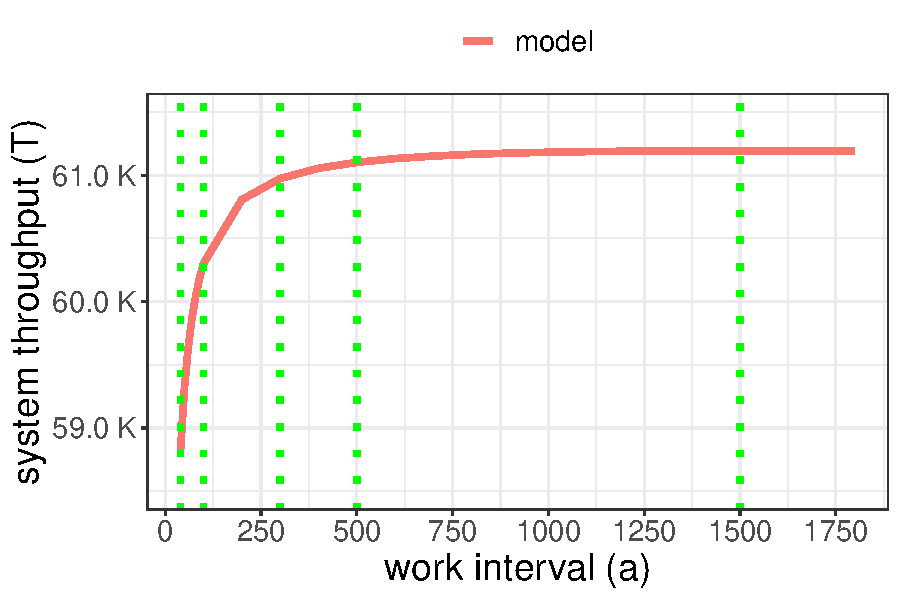
\includegraphics[width=\linewidth]{figures/fig-7.pdf}
  \captionof{figure}{System throughput estimates $vs.$ $a$.  
    Green dotted lines indicate regions with different gradients (as discussed in \Cref{{sec:determ-optim-ep}}).}
  \label{fig:7} 
\end{minipage}
\end{figure*}

\begin{figure*}[hbt!]
    \centering
    \begin{subfigure}{0.49\textwidth}
        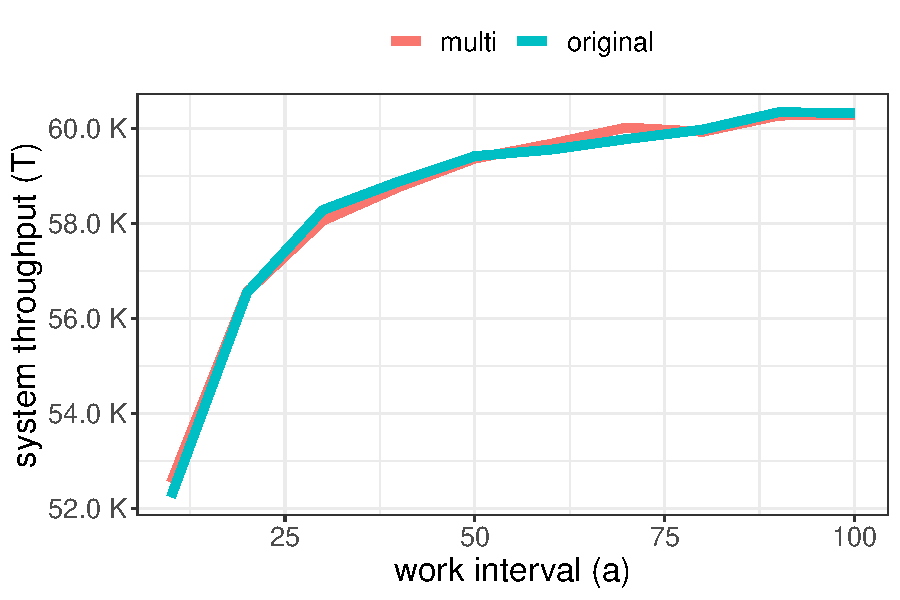
\includegraphics[width=\linewidth]{figures/fig-8a.pdf}
        \captionof{figure}{Simulations using paired affinity.} \label{fig:8a}
    \end{subfigure}%
    \hspace*{\fill}   
    \begin{subfigure}{0.49\textwidth}
        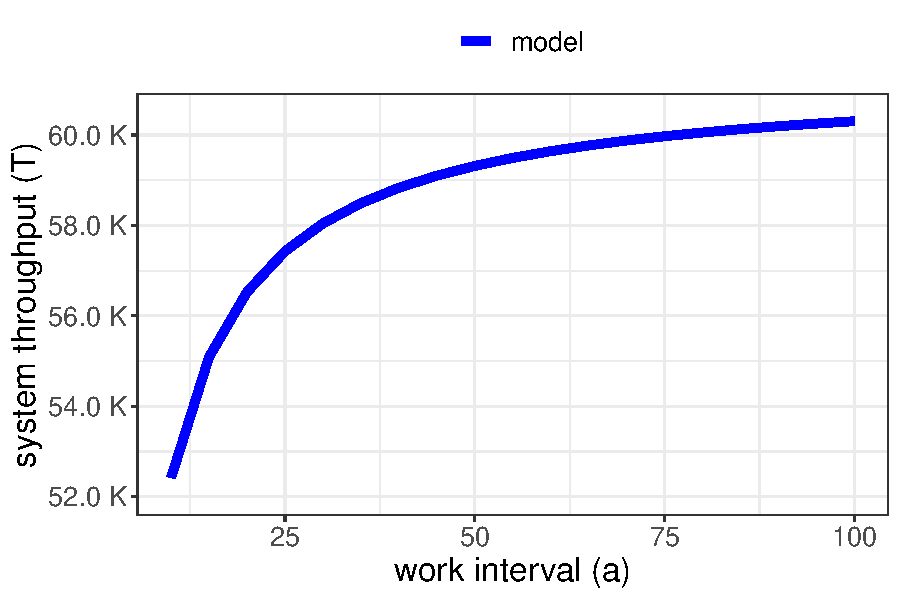
\includegraphics[width=\linewidth]{figures/fig-8b.pdf}
        \captionof{figure}{Model using random affinity.} \label{fig:8b}
    \end{subfigure}
    \caption{Maximum throughput as work interval $a$ varied from 10 to 100 $ms$.} \label{fig:8}
\end{figure*}

\begin{figure*}[h!tb]
    \centering
    \begin{subfigure}{0.49\textwidth}
        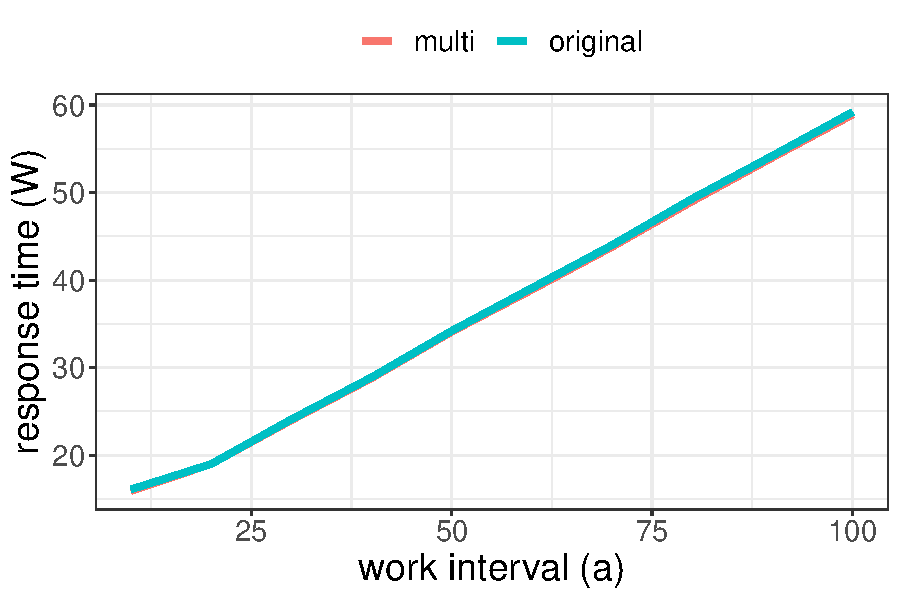
\includegraphics[width=\linewidth]{figures/fig-9a.pdf}
        \caption{Simulations with paired affinity as $a$ is varied from 10 to 100 $ms$ 
        ($\lambda = 40,000$).} \label{fig:9a}
    \end{subfigure}%
    \hspace*{\fill}   
    \begin{subfigure}{0.49\textwidth}
        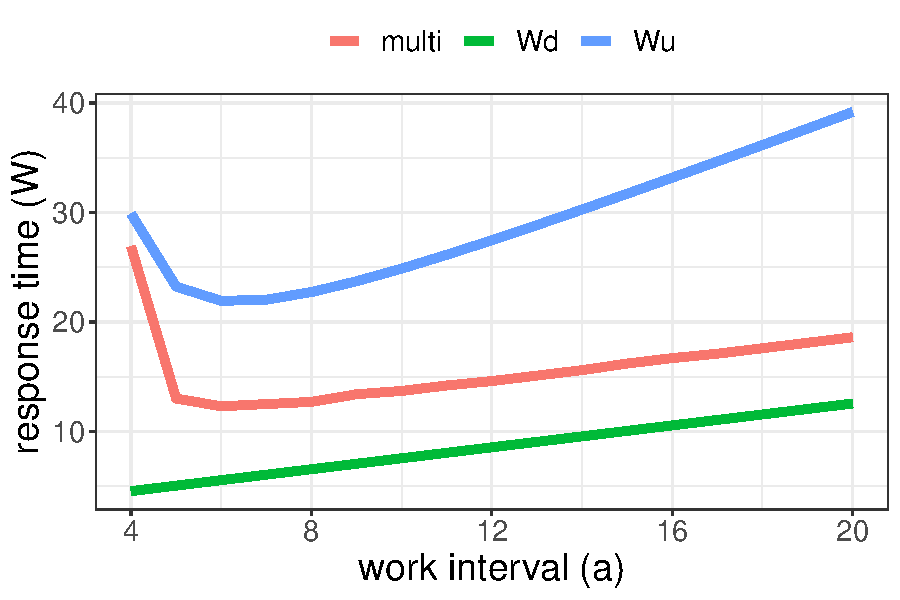
\includegraphics[width=\linewidth]{figures/fig-9b.pdf}
        \caption{Multi-commit with paired affinity and models with random affinity as $a$ is varied from 4 to 20 $ms$ ($\lambda = 30,000$).} \label{fig:9b}
    \end{subfigure}
    \caption{Average response time (ms).} \label{fig:9}
\end{figure*}
